\documentclass{template/openetcs_report}
% Use the option "nocc" if the document is not licensed under Creative Commons
%\documentclass[nocc]{template/openetcs_report}
\usepackage{url}
\usepackage{hyperref}
\usepackage{listings}
\usepackage{float}
\usepackage{lscape}
\graphicspath{{./template/}{.}{./images/}}


%New command

\newcommand\refFigure[1]{figure~\ref{#1}, page~\pageref{#1}}
\newcommand\refChapter[1]{chapter~\ref{#1}}
\newcommand\refTable[1]{table~\ref{#1}}
\newcommand\packageName[1]{\emph{#1}}


\begin{document}
\frontmatter
\project{openETCS}

%Please do not change anything above this line
%============================
% The document metadata is defined below

%assign a report number here
\reportnum{OETCS/WP7/O??}

%define your workpackage or task here
\wp{openETCS@ITEA Work Package 7: ``Toolchain''}

%set a title here
\title{Evaluation model of ETCS using SysML and Enterprise Architect}

%set a subtitle here
\subtitle{Tool and model presentation}

%set the date of the report here
\date{March 2013}

%define a list of authors and their affiliation here
\author{Thomas Bardot}

\affiliation{Mitsubishi Electric R\&D Centre Europe\\
1 allée de Beaulieu\\
CS 10806\\
35708 RENNES cedex 7\\
\\
email: \url{t.bardot@fr.merce.mee.com}
}

% define the coverart
\coverart[width=350pt]{openETCS_EUPL.png}

%define the type of report
\reporttype{Draft Report}


\begin{abstract}
%define an abstract here
  FIXME
\end{abstract}

%=============================
%Do not change the next three lines
\maketitle
\tableofcontents
\listoffiguresandtables
%=============================
% The actual document starts below this line
%=============================

%Start here
\mainmatter

%Examples are below

%=============================
% INTRODUCTION
%=============================

\chapter{Introduction}
This document describes a SysML model of the ETCS SRS SUBSET-026-3.5.3 \cite{SRS}. An overview of the formalism and of the SysML model is given. Then, we discuss about the benefits and shortcomings of the formalism and the modeling strategy. In order to make the model easier to understand, a detailed description of the model with explanations is given.

\section{Formalism and tool description}
\subsection{SysML} \label{SysML}

The System Modeling Language (SysML) is a graphical language based on an Unified Modeling Language (UML) profile. It represents a subset of UML 2.0 with extensions needed to model complex systems with hardware, software, procedures and many other elements. 
SysML uses nine kind of diagrams which allow to model requirements, parameters relationship, structure and behavior of a system. These diagrams are the following:

\begin{itemize}
	\item Activity diagram;
	\item Block definition diagram;
	\item Internal block diagram;
	\item Package diagram;
	\item Parametric diagram;
	\item Requirement diagram;
	\item Sequence diagram;
	\item State machine diagram;
	\item Use case diagram.
\end{itemize}

SysML diagrams are structured as shown in \refFigure{fig:SysML_Diagram_Types}.

\begin{figure}[h]
  \centering
  \fbox{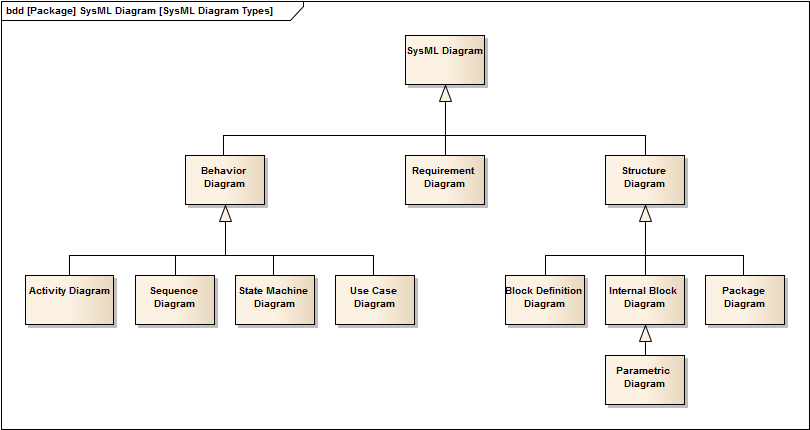
\includegraphics[width=6in]{SysML_Diagram_Types}}
  \caption{SysML diagram types}
  \label{fig:SysML_Diagram_Types}
\end{figure}

\subsection{SysML tools}

There are many tools supporting SysML, open source or not. Most common open source tools are Topcased and Papyrus, based on the Eclipse Platform. 

We tried Topcased, but we faced problems, including a corrupted project file. We also had problem when changing the diagram hierarchy : when trying to allocate an existing diagram (bdd) into another object by using the outline view, nothing happened, the \textsl{.xmldi} file seems to not be properly updated. We noticed an important memory consumption (up to 1GB), probably due to the Eclipse Platform, that could cause the crash of the tool. 

Thus, we chose to use Enterprise Architect v10, a tool under a proprietary license edited by Sparx System. It has the advantages to be one of the cheapest proprietary SysML tool. Among its characteristics, Enterprise Architect has a model simulator that permits to simulate behavioral diagram step by step. It also has a code generator that permits to translate diagrams and SysML elements into code in ADA, C/C++, java and other languages. These characteristics could be interesting for further studies about the development of a model simulator. Sparx System claims that Enterprise Architect has a good scalability. Our model is too light to confirm this assertion, but we notice a low memory consumption compared with Topcased, and the tool remains reactive.

\section{Model purpose}

Our work consisted in modeling the SRS SUBSET-026-3.5.3 \cite{SRS}: ``Establishing a communication session'', only when the communication is initiated by the OBU. The purposes of this work is to realize a behavioral model of this ETCS function. The model shall contain all the information states in the  [TODO add ref] SRS SUBSET-026-3.5.3, and it shall be easy to access to this information by reading the model. An important point is that the model shall be well structured in order to help its comprehension and verification. The model should also include traceability information.

%=============================
% MODEL OVERVIEW
%=============================

\chapter{Model overview}


%=============================
% Diagram choice
\section{Diagram choice}

As seen in \refChapter{SysML}, behavioral model can be based on state machine diagram, activity diagram, sequence diagram or use case diagram. A model evaluation with SysML state machine diagrams is already done by Cécile Braunstein \cite{Braunstein_SysML_Model}, so we prefer to evaluate other way to model system behavior. Use case diagram has a too high-level view of the system in order to model detailed functional behavior. Sequence diagram may fit better to the modeling of the SRS SUBSET-026-3.5.3, but it is a particular approach, service-oriented, which may not be relevant to model other ETCS functions.

Therefore, our behavioral model is based mostly on the activity diagram. Activity diagram may describe a behavior by the transformation of inputs to outputs through a controlled sequence of actions. An activity can also depict the behavior performed by a block or a part. Thus, this kind of diagram permits to show the relationship between block inputs and outputs, and to clearly identify the processing performed by a block or a part.

We also used requirement diagram and block definition diagrams in order to collect requirements and to structure our model. Notice that if we had to model more precisely the logical structure of the ETCS functions, we would also use the internal block diagram.

%=============================
% Modeling strategy
\section{Modeling strategy} \label{Modeling_strategy}

The modeling strategy is represented by the \refFigure{fig:Modeling_strategy}.

First of all, the modeling activity started with the definition of all the requirements applicable to the function \textsl{Establishing Communication Session}. These requirements simply represent the SRS SUBSET-026-3.5.3 \cite{SRS} which is split into basics requirements.

Then a brief logical structure of the \textsl{Manage Communication Session} functions is made by using blocks and parts.
An activity is associated to the block \textsl{Establishing Communication Session} and represents its behavior. This activity call other activities which permits to break down the model complexity and to help its comprehension.

In conjunction with the activity modeling, data types are defined by using enumeration and signals.

\begin{figure}[h]
  \centering
  \fbox{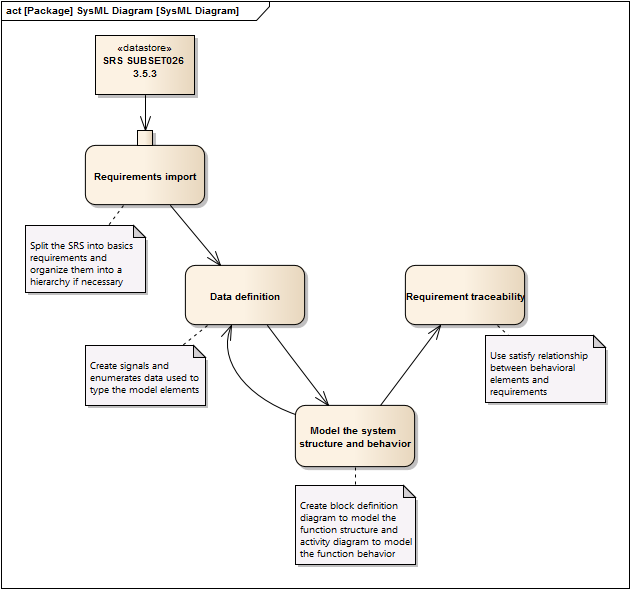
\includegraphics[width=5in]{Modeling_strategy}}
  \caption{Schematic representing the methodology used}
  \label{fig:Modeling_strategy}
\end{figure}

%=============================
% Modeling structure
\section{Modeling structure}

The model is composed of three main packages:
\begin{itemize}
	\item \packageName{Data} package which contains block definition diagrams where enumeration and signals are defined;
	\item \packageName{System requirements} package;
	\item \packageName{System behavior and structure} package.
\end{itemize}

 The \packageName{system behavior and structure} package imports the \packageName{System requirements} and \packageName{data} packages as shown by the \refFigure{fig:Model_overview}.

\begin{figure}[h]
  \centering
  \fbox{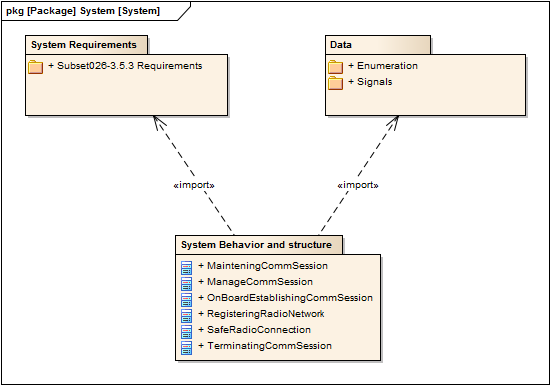
\includegraphics[width=4in]{Model_overview}}
  \caption{Overview of the SysML model structure}
  \label{fig:Model_overview}
\end{figure}

\subsection{\packageName{Requirements} package}

As explains in \refChapter{Modeling_strategy}, this package contains requirement diagram where all the requirements applicable to the \textsl{Establish a communication session} function are shown. All these requirements simply represent the text of the SRS SUBSET-026-3.5.3 \cite{SRS}, when each requirement represents an elementary part of it. 

Because creating manually all these requirements is too long, we generate them by importing a \textsl{.csv} file with the format described in the \refTable{tab:CsvFileFormat}. The \emph{Type} field is a mandatory field that must match Enterprise Architect element types : requirement or package in our use case. In order to organize the model, it is important to import a package and indicate where the imported requirements have to be placed. The model hierarchy is then created with the \emph{CSV\_KEY} and \emph{CSV\_PARENT\_KEY} fields. A key consists in a unique identifier for each element.

\begin{table*}
	\begin{center} \scriptsize
		\begin{tabular} {|p{3.7cm}|p{2cm}|p{3cm}|p{2.8cm}|p{2.8cm}|}
		\hline
			
			\textbf{NAME}&\textbf{TYPE}&\textbf{NOTE}&\textbf{CSV\_KEY}&\textbf{CSV\_PARENT\_KEY} \\
			
			\textsl{Name of the element to be imported}&\textsl{type of the element (package or requirement)}&\textsl{Description of the element}&\textsl{Id of the element, same as the element's name}&\textsl{Id of the hierarchical parent} \\ \hline
			
			Subset026-3.5.3 Requirements&package&Establishing a communication session&Subset026-3.5.3 Requirements& \\ 
			
			REQ\_SRS026\_3.5.3.4&	Requirement&	The on-board shall establish a communication session&	REQ\_SRS026\_3.5.3.4&	Subset026-3.5.3 Requirements \\ 
			
			REQ\_SRS026\_3.5.3.4-1&	Requirement&	a) At Start of Mission (only if level 2 or 3).&	REQ\_SRS026\_3.5.3.4-1&	REQ\_SRS026\_3.5.3.4\\
			
		\hline
		\end{tabular}
	\end{center}
	\caption{format of the .csv file used to import requirements}
	\label{tab:CsvFileFormat}
\end{table*}

Because each requirement represents an elementary part of the SRS text, we try as far as possible to not insert hierarchical dependencies between requirements. Nevertheless, we did it when the SRS specifies a list of conditions that shall be met in order to fulfill a need. In this case, all the requirements corresponding to the conditions are contained into a parent requirement which represents the need to fulfill. The \refTable{tab:CsvFileFormat} show an example of this case. Requirement name is made on this pattern : REQ\_SRS026\_\emph{chapter}.

\subsection{\packageName{Data} package}

The \packageName{data} package contains block definition diagrams where enumerations and signals are defined (see \refChapter{chap:DataPackage}). These data types are used in the model to type the different SysML elements like connectors, ports, action pins, activity parameters, attributes or operation arguments. 

We choose to use signals to model structured data exchanged between blocks or activities. Indeed, SysML definition of signal is \cite{SysML_Guide}: ``A signal defines a message that can be sent and received by a block. It has a set of attributes that specify the content of the message''. Then, in our model, a signal element represent a message, and signal attributes represents the message contents. An attribute can be typed with a primitive value (e.g. boolean, integer) or with an enumerate.

\subsection{\packageName{System Behavior and structure} package}

The \packageName{system behavior and structure} package contains the block definition diagram which describes the functions logical structure (see \refFigure{fig:System_Behavior}). The physical ETCS structure, for example with an on-board block and a trackside block, is not represented. Thus, blocks only represent ETCS functions or sub-functions which apply to any physical part of the ETCS system. 

In our model, we create a block \textsl{OnBoardEstablishingCommSession}. It represents the function \textsl{Establishing Communication Session} described in the SRS SUBSET-026-3.5.3, only in the case where OBU is initiating the communication session. But, the behavior on this function cannot be allocated to a particular physical sub-system like the OBU. In fact, this function describes the behavior of different ETCS sub-systems (OBU, RIU or RBC) when the OBU is initiating the communication session. 

A block may have attributes or operations. Block attributes should represent information relevant to the block behavior that has to be stored. It can be block states, or constants for example. A block operation defines in our model a basic logical function used to describe a small part of the block behavior. It permits to reduce the complexity and to increase the readability of the behavior diagrams by calling operations. But, on the other hand, diagrams contain less information.

\packageName{System behavior and structure} package also contains the activity diagrams which depict the function behavior. System behavior and system logical structure are in the same package because it helps to link activity to their owner block and improves the model hierarchy.

An activity is associated to the block \textsl{OnBoardEstablishingCommSession} and depict its behavior (see \refFigure{fig:EstablishCommSession}). This activity has the same name than this block. The inputs and outputs parameters of this activity represents the inputs and outputs of its owner block. 

Even if it is not mandatory, our activity diagrams consists in a sequence of actions related by control relationship and this sequence is delimited by an initial node and a final node. It is justified because each activity that we use represents a specific  process limited in time with states and not just a never-ending process on a stream.

An activity can call other sub activities. In order to do that, we chose to use call behavior actions. These actions may have some input or output pins corresponding to the input and output parameters of the activity which they call. The connection between activity parameters and action pins is often hidden for a better diagram readability. But we notice that the tool does not provide layers in order to easily hide or show the connectors or another specific part of a diagram.

As mentioned before, an activity can call operations defined in a block. It is done by using a call operation action. The operation input parameters are linked to the action input pins. The operation result is linked to the action output pin.

Activities use decision element that indicates a point of conditional progression: if a condition is true, then processing continues one way; if not, then another. The condition is made by evaluating a variable. This variable often consists in an output pin of a call operation action. So, we assume that an action pin, or an activity parameter, or a block port can be seen as a variable with the same name. We also assume that a connection between two of these elements can be seen as an assignment of the target element with the value of the source element. 


%=============================
% MODEL BENEFITS AND SHORTCOMMINGS
%=============================

\chapter{Model benefits and shortcomings}

Using SysML with Enterprise Architect in order to model a SRS chapter presents some benefits and shortcomings which are listed below.

%=============================
% Benefits
\section{Benefits}

From our point of view, using SysML provides these benefits:

\begin{itemize}
\item It is a graphical language easy to understand even to people who are not intimate with this method;
\item SysML allows to represent different views of a system, for example a requirements view with requirements diagrams, a view of the system structure with block definition diagram, a view of the system behavior with states machines or activity diagrams, and a view of the system constraints with the parametric diagrams.
\end{itemize}

From our point of view, Enterprise Architect SysML tool provides these benefits:

\begin{itemize}
\item Code generation and behavior simulation;
\item Many examples and a useful learning center are provided with the tool;
\item The tool seems stable and scalable.
\end{itemize}

%=============================
% Shortcomings
\section{Shortcomings}
SysML doesn't have a strong semantic, therefor when modeling a system, the developer faces several modeling choices. For example, when modeling the data exchange between activities, we had the choice between using send signal action or pass through outputs and inputs activities parameters. These choices have their own advantages and defects. So it is important to set a subset of SysML applicable to the OpenETCS project and to define our semantic.

As mentioned previously, because SysML is a graphical language, it is easy to understand. But it implies that all the model information cannot be on the model diagram. Indeed, if diagram contains to much graphical information, it would become not understandable at all. The requirements management is a good example of this point of view. Requirement diagrams are useful to show dependencies between requirements, but it becomes useless when a lot of requirements are imported to the model. Moreover, using the \emph{satisfy} relationship by drawing a connector between all the model elements and the satisfied requirements can make the diagram not readable, thus the use of a cross-check matrix could be more relevant.


Enterprise Architect allows model code generation or model simulation. But we need to create a particular model in order to be able to generate code or simulate it. The model simulation permits to simulate states machines or activities one by one. But we did not find how to simulate several activities diagrams running concurrently.


%=============================
% DETAILED MODEL DESCRIPTION	
%=============================

\chapter{Detailed model description} \label{Detailed_model}

This chapter gives all the diagrams used by our model. But, because all the model information can't stand only on diagrams, please refer to the automatically generated \emph{ModelDocumentation.pdf} for a full model description.

%=============================
% Requirements package
\section{\packageName{Requirements} package}

\begin{figure}[H]
  \centering
  \fbox{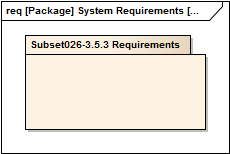
\includegraphics[width=2in]{System_Principles_Req}}
  \caption{Req diagram containing packages for each ETCS chapter}
  \label{fig:System_Principles_Req}
\end{figure}

\begin{figure}[H]
  \centering
  \fbox{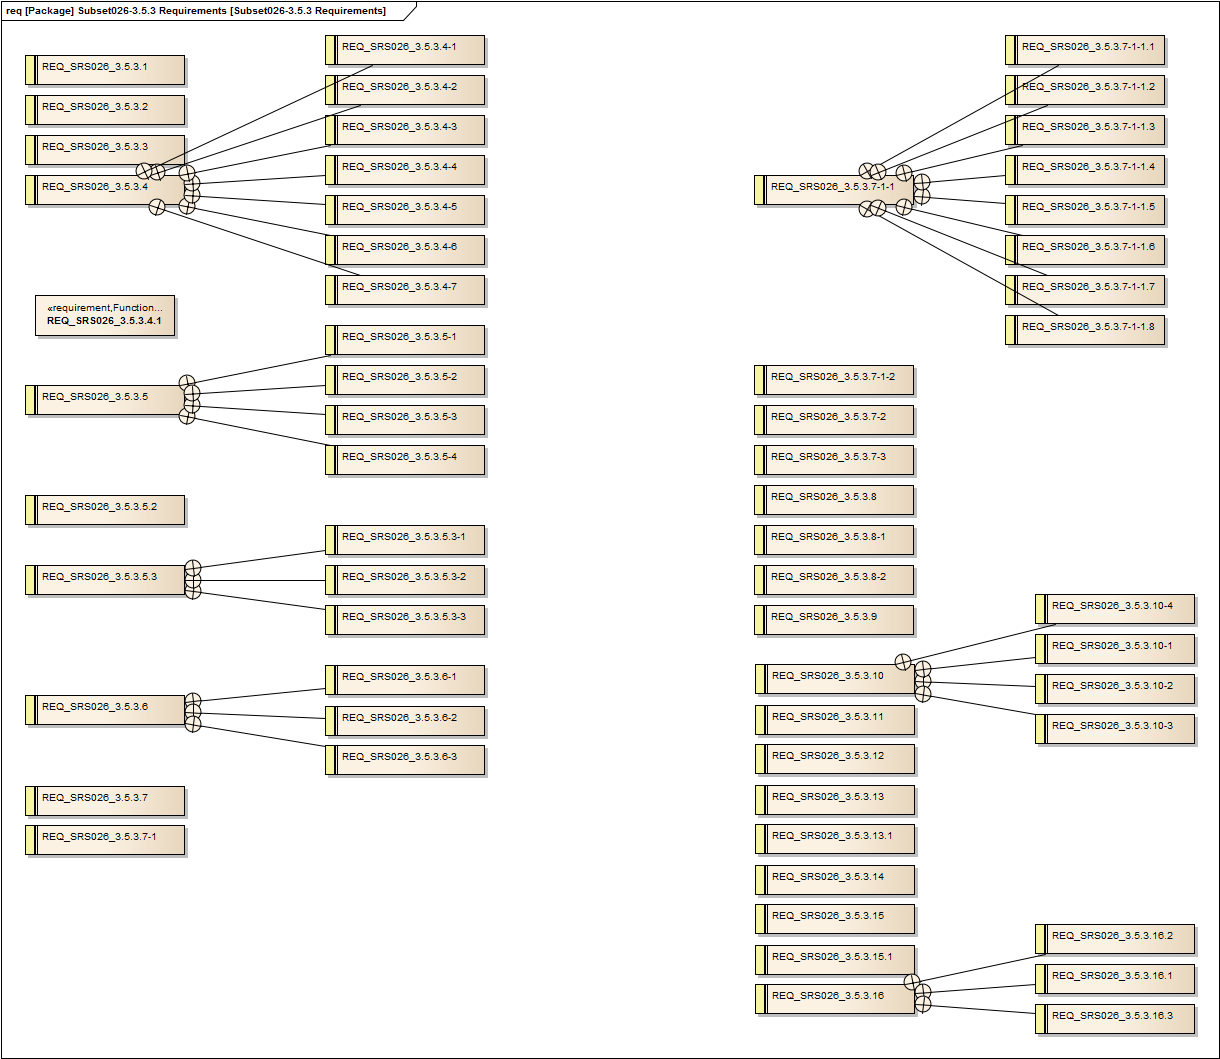
\includegraphics[width=6in]{Subset026-353_Requirements}}
  \caption{Req diagram containing the requirements corresponding to the SRSSYBSET026 3.5.3}
  \label{fig:Subset026-3.5.3_Requirements}
\end{figure}

%=============================
% data package
\section{\packageName{Data} package} \label{chap:DataPackage}

\begin{figure}[H]
  \centering
  \fbox{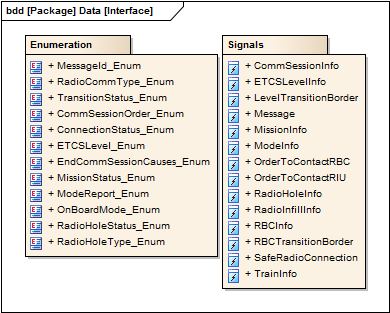
\includegraphics[width=3in]{Interface}}
  \caption{Bdd diagram containing packages for each data type (enumeration or signal)}
  \label{fig:Interface}
\end{figure}

\begin{figure}[H]
  \centering
  \fbox{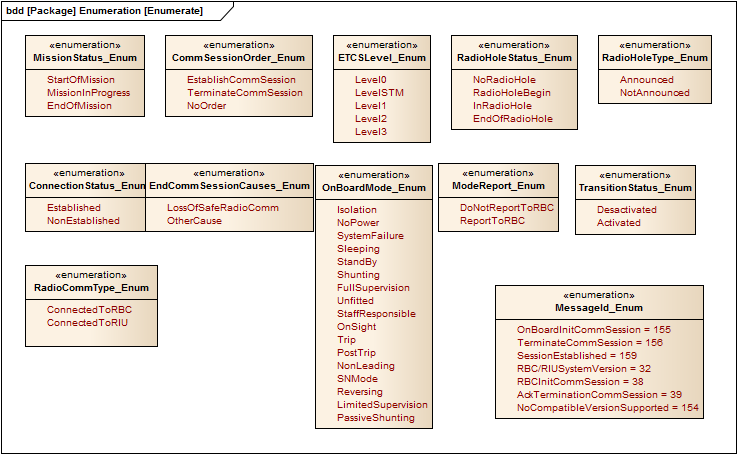
\includegraphics[width=6in]{Enumerate}}
  \caption{Bdd diagram containing the definition of the enumerates used by the model}
  \label{fig:Enumerate}
\end{figure}

\begin{figure}[H]
  \centering
  \fbox{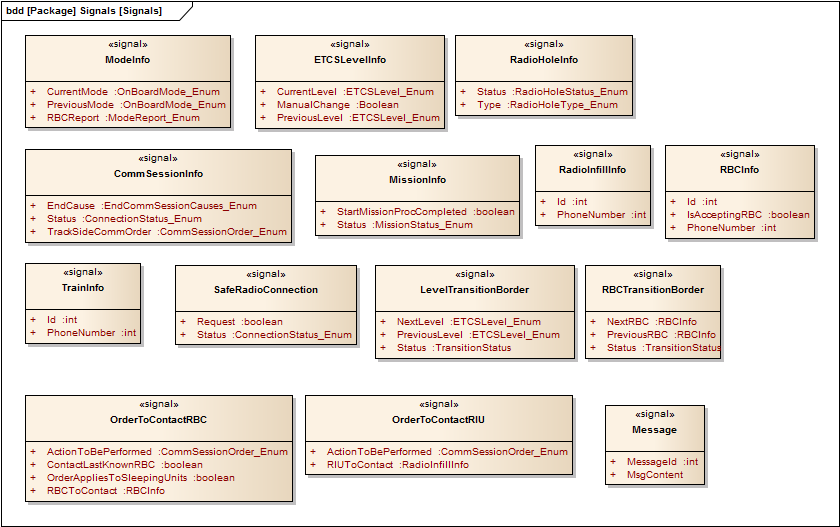
\includegraphics[width=6in]{Signals}}
  \caption{Bdd diagram containing the definition of the signals used by the model}
  \label{fig:Signals}
\end{figure}

%=============================
% System Behavior and structure package
\section{\packageName{System Behavior and structure} package}

\begin{figure}[H]
  \centering
  \fbox{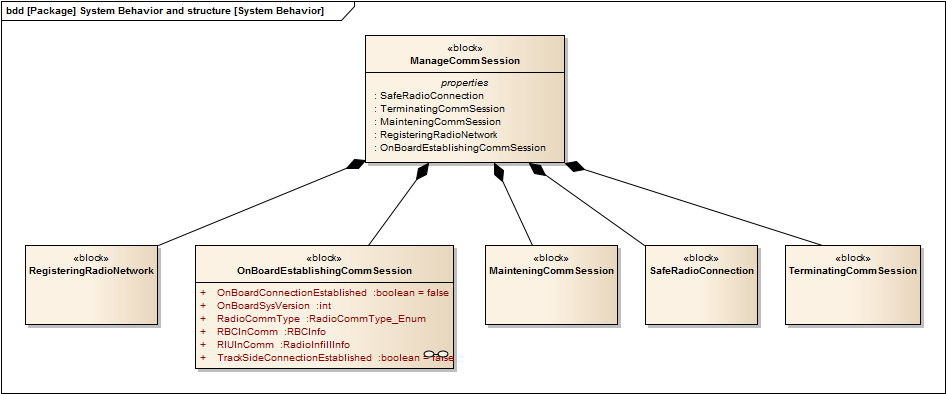
\includegraphics[width=5in]{System_Behavior}}
  \caption{Bdd diagram containing blocks which provide a very brief description of the function structure}
  \label{fig:System_Behavior}
\end{figure}

\begin{figure}
  \centering
  \fbox{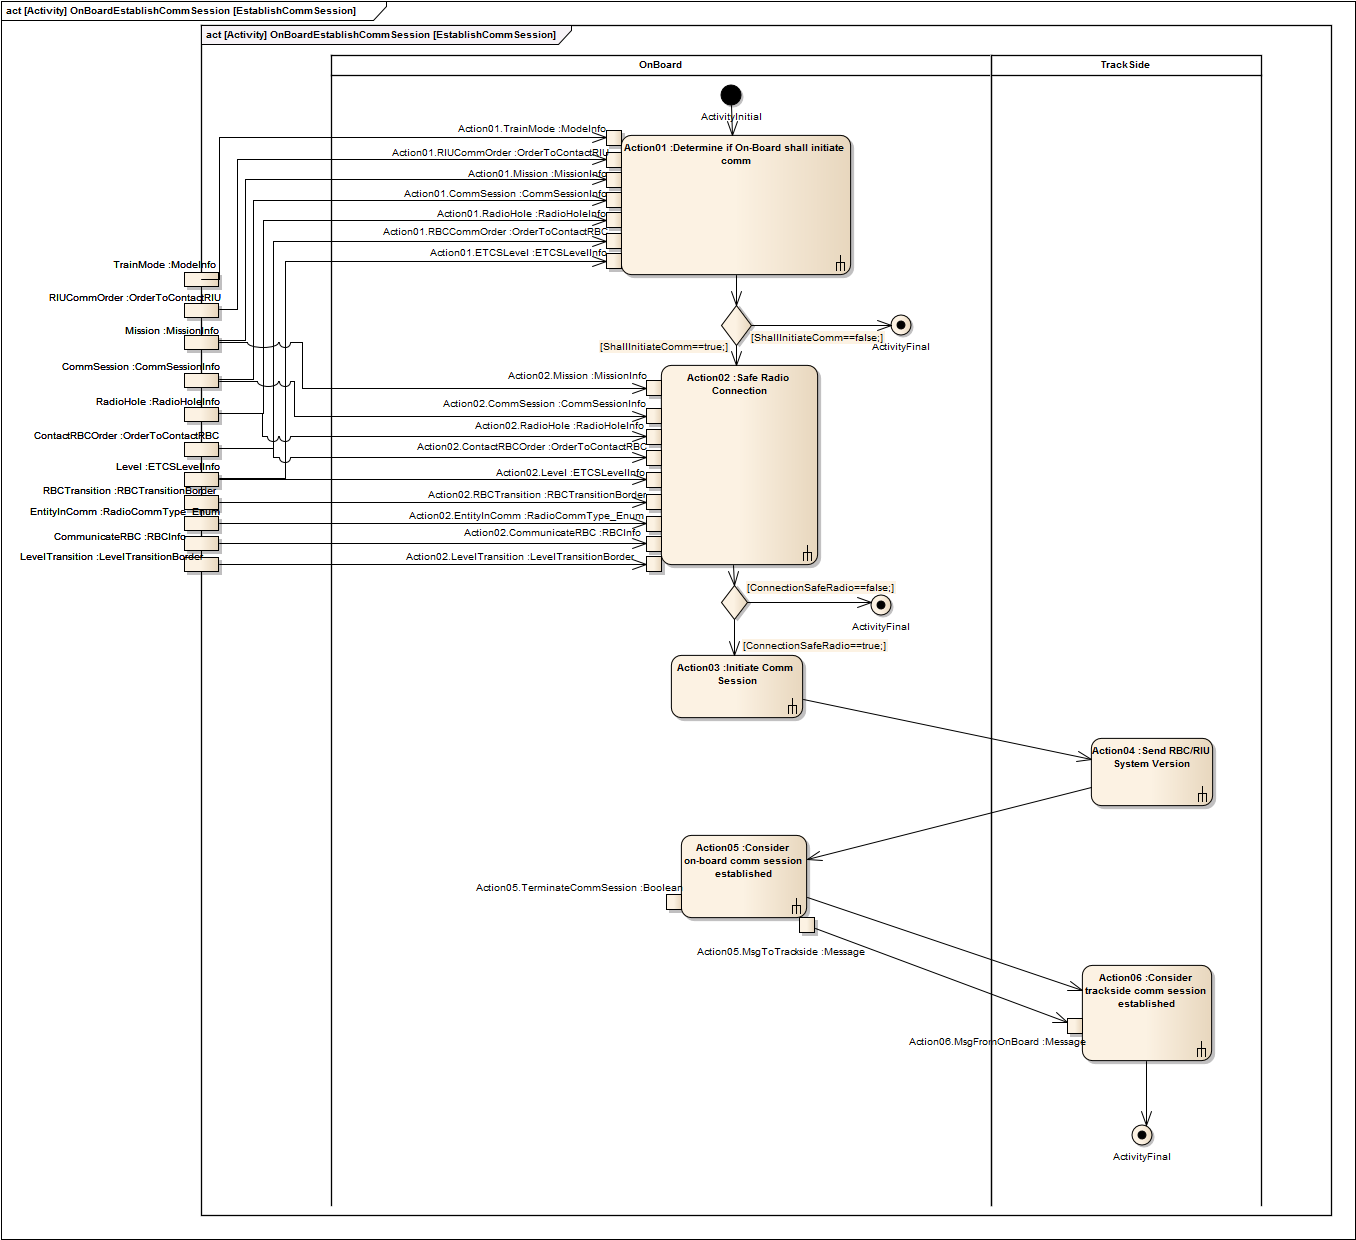
\includegraphics[width=7in]{EstablishCommSession}}
  \caption{Main activity diagram describing the behavior of the block \emph{OnBoardEstablishingCommSession}}
  \label{fig:EstablishCommSession}
\end{figure}

\begin{landscape}
\begin{figure}
  \centering
  \fbox{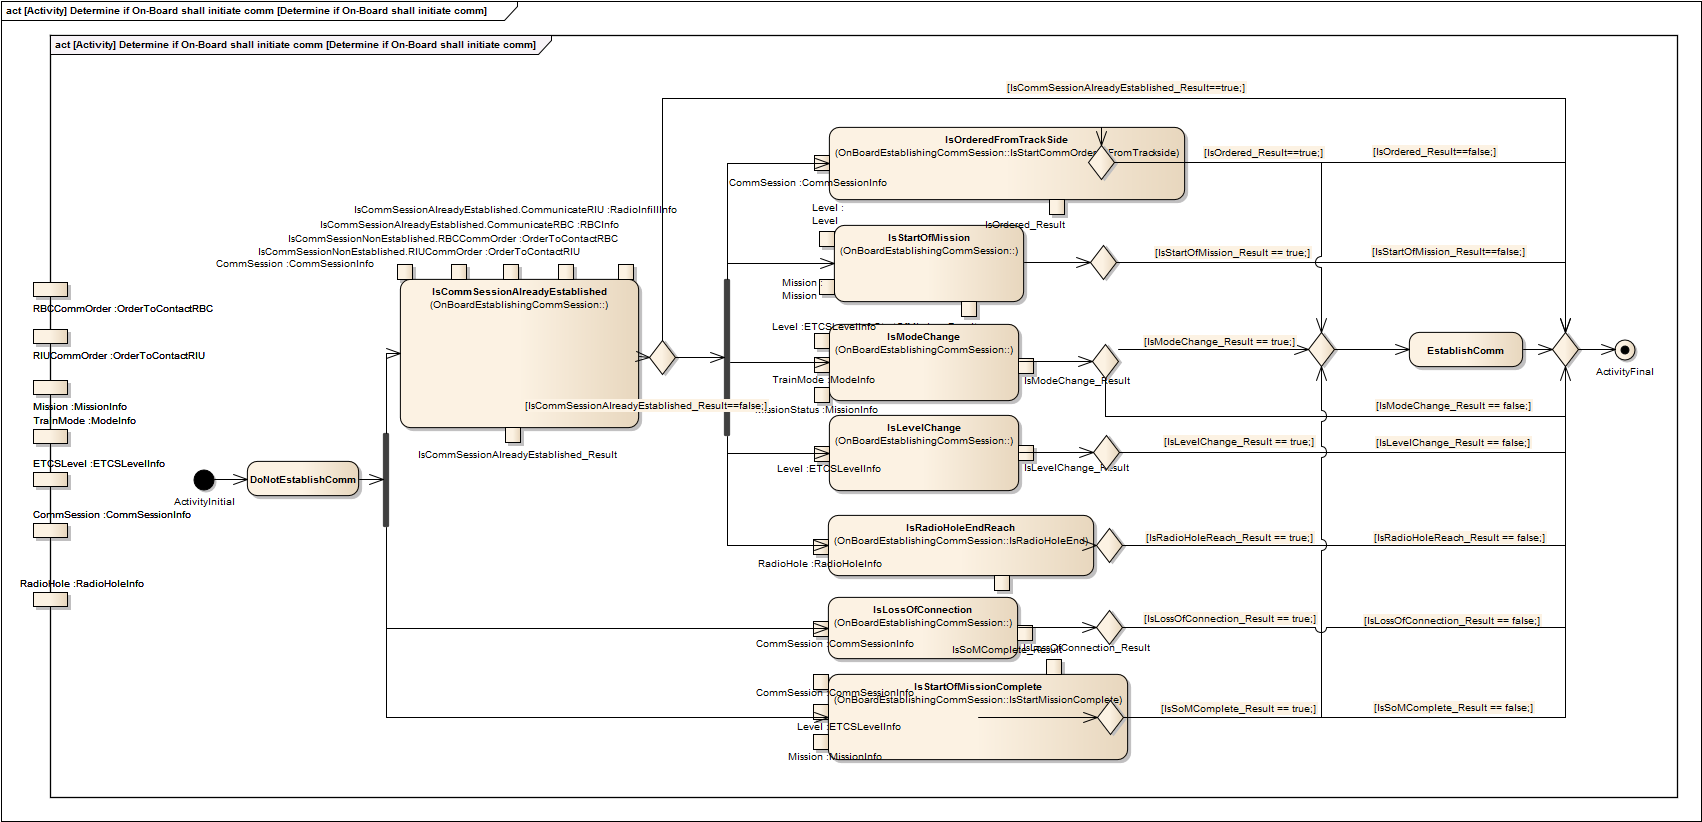
\includegraphics[width=9.5in]{Determine_if_On-Board_shall_initiate_comm}}
  \caption{Activity diagram describing how the on-board determines if it may establish a communication session}
  \label{fig:Determine_if_On-Board_shall_initiate_comm}
\end{figure}
\end{landscape}

\begin{figure}
  \centering
  \fbox{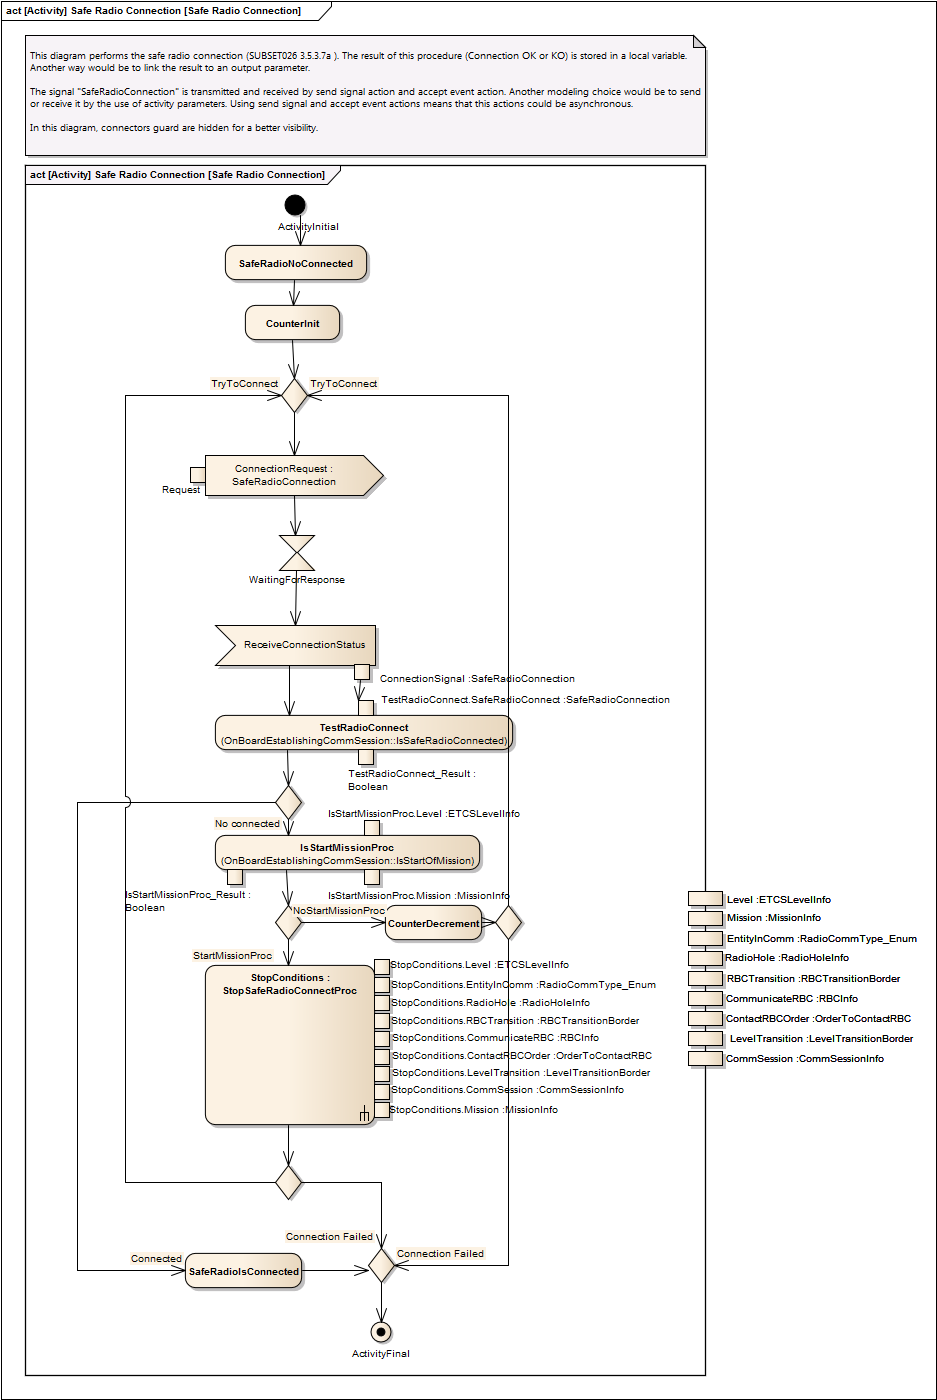
\includegraphics[width=6in]{Safe_Radio_Connection}}
  \caption{Activity diagram describing how the on-board shall establish a safe radio connection}
  \label{fig:Safe_Radio_Connection}
\end{figure}

\begin{figure}
  \centering
  \fbox{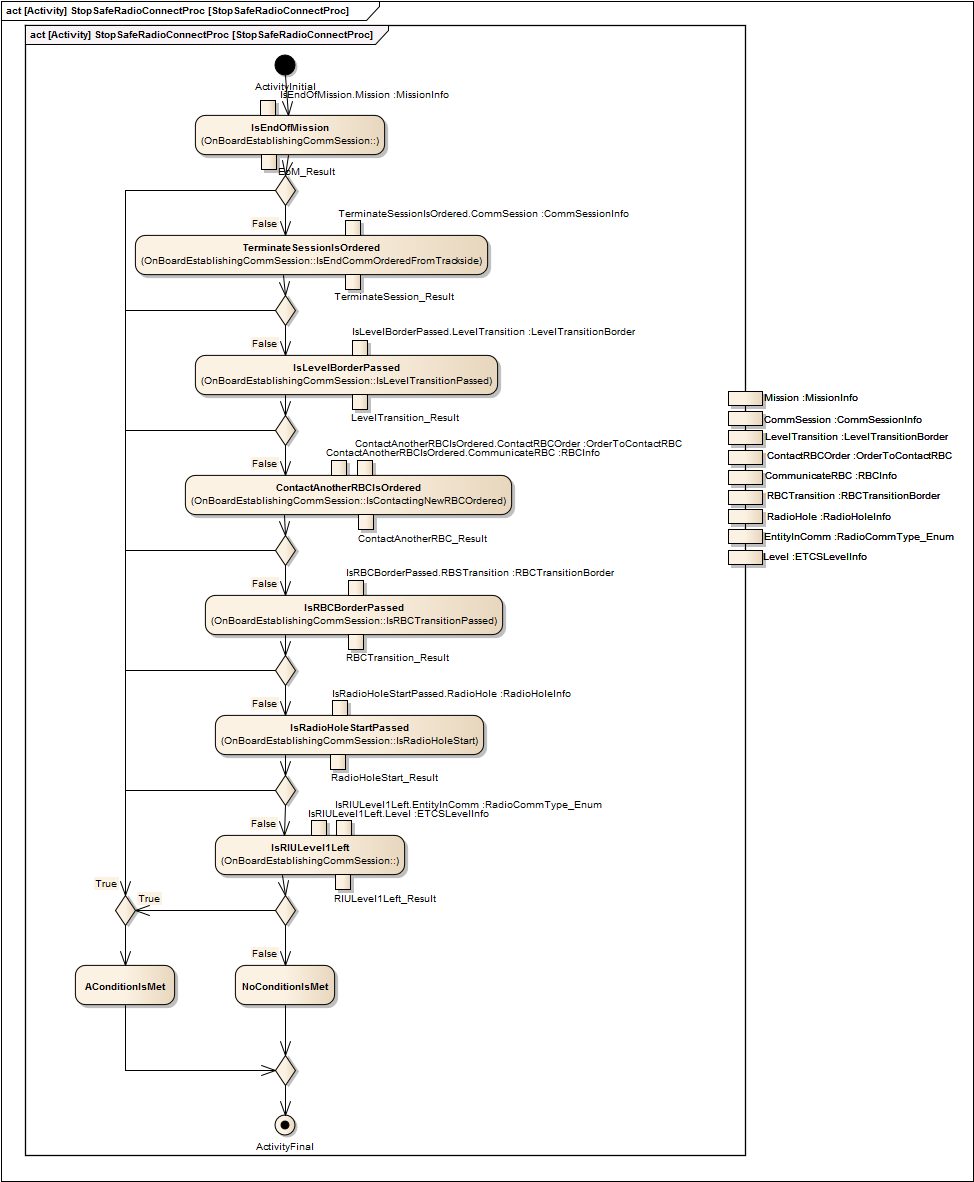
\includegraphics[width=6in]{StopSafeRadioConnectProc}}
  \caption{Activity diagram describing how the on-board shall abort the safe radio connection process}
  \label{fig:StopSafeRadioConnectProc}
\end{figure}

\begin{figure}
  \centering
  \fbox{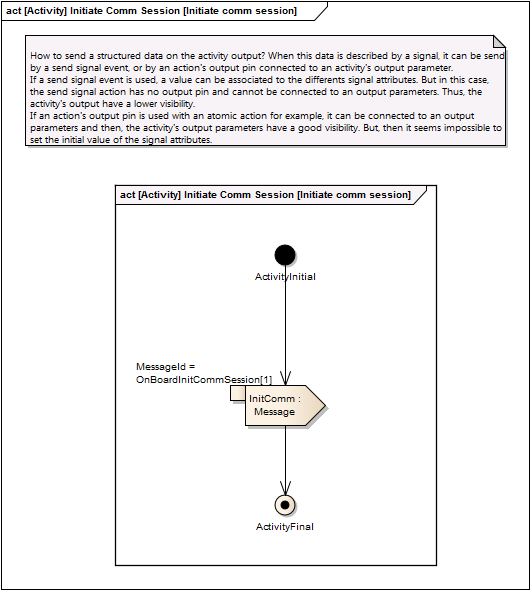
\includegraphics[width=4in]{Initiate_comm_session}}
  \caption{Activity diagram describing the initialization of a communication session by the on-board}
  \label{fig:Initiate_comm_session}
\end{figure}

\begin{figure}
  \centering
  \fbox{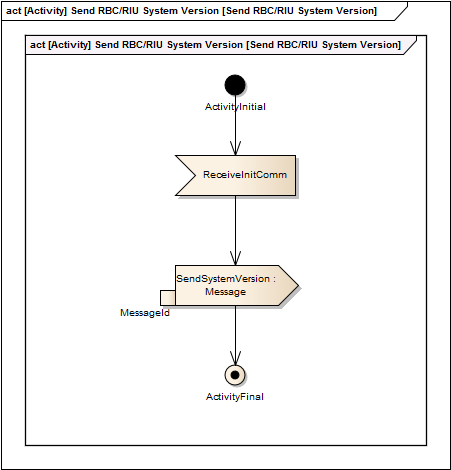
\includegraphics[width=4in]{Send_RBCRIU_System_Version}}
  \caption{Activity diagram describing the trackside response to an initialization of communication session by the on-board}
  \label{fig:Send_RBCRIU_System_Version}
\end{figure}

\begin{figure}
  \centering
  \fbox{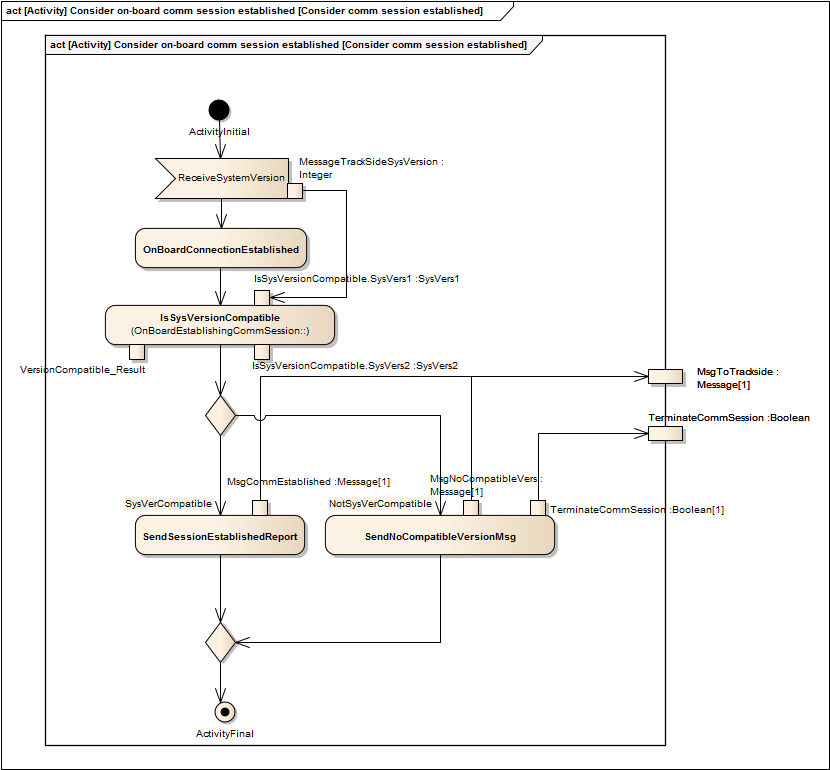
\includegraphics[width=6in]{Consider_comm_session_established}}
  \caption{Activity diagram describing the on-board behavior when it receives the RBC/RIU system version}
  \label{fig:Consider_comm_session_established}
\end{figure}

\begin{figure}
  \centering
  \fbox{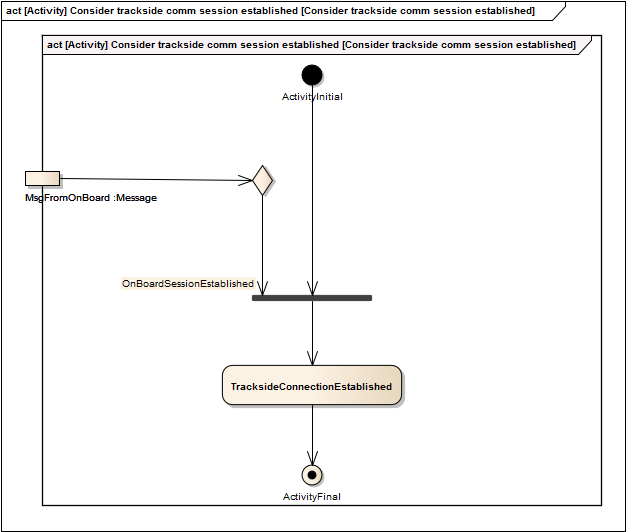
\includegraphics[width=5in]{Consider_trackside_comm_session_established}}
  \caption{Activity diagram describing the trackside behavior when communication session is established by the on-board}
  \label{fig:Consider_trackside_comm_session_establishedd}
\end{figure}



%\begin{figure}
% \centering
%  \fbox{
\includegraphics[width=2in]{itea}}
%  \caption{Yet Another Castle In Appendix}
%  \label{fig:castle2}
%\end{figure}

%=============================
% BIBLIOGRAPHY	
%=============================

\bibliographystyle{abbrv}
\bibliography{bibliography-sample-merce}

%===================================================
%Do NOT change anything below this line

\end{document}
